\documentclass[10pt,letterpaper,oneside]{article}
\usepackage[T1]{fontenc}
\usepackage[utf8]{inputenc}
\usepackage{lmodern}
\usepackage{geometry}
\geometry{margin=0.84in,headheight=21pt,footskip=28pt}
\usepackage{microtype}
\usepackage{xcolor}
\definecolor{ink}{HTML}{15253D}
\definecolor{accent}{HTML}{086A84}
\definecolor{pale}{HTML}{EEF5F8}
\definecolor{muted}{HTML}{4E6474}
\definecolor{grayline}{HTML}{D7E2E8}
\usepackage{graphicx}
\usepackage{fancyhdr}
\usepackage{titlesec}
\usepackage{enumitem}
\usepackage{array,tabularx,longtable,booktabs}
\usepackage[most]{tcolorbox}
\usepackage{xurl}
\usepackage{hyperref}
\usepackage{listings}
\usepackage{amsmath,amssymb}
\usepackage{tikz}
\usetikzlibrary{arrows.meta,positioning,shapes.geometric,calc}
\hypersetup{colorlinks=true,linkcolor=accent,urlcolor=accent,pdftitle={Security Foundations and Threat Modeling},pdfauthor={Independent technical engineering study companion}}
\renewcommand{\familydefault}{\sfdefault}
\linespread{1.07}
\setlength{\parindent}{0pt}
\setlength{\parskip}{5.5pt}
\emergencystretch=2em
\setlist[itemize]{leftmargin=1.5em,itemsep=2.5pt,topsep=3pt}
\setlist[enumerate]{leftmargin=1.7em,itemsep=3pt,topsep=3pt}
\titleformat{\section}{\Large\bfseries\color{ink}}{\thesection}{0.65em}{}[\vspace{-2pt}{\color{accent}\titlerule}]
\titleformat{\subsection}{\large\bfseries\color{accent}}{\thesubsection}{0.6em}{}
\titleformat{\subsubsection}{\bfseries\color{ink}}{\thesubsubsection}{0.6em}{}
\titlespacing*{\section}{0pt}{16pt}{9pt}
\titlespacing*{\subsection}{0pt}{11pt}{6pt}
\pagestyle{fancy}\fancyhf{}\fancyhead[L]{\footnotesize\color{muted} COMPUTER \& INFORMATION SECURITY ENGINEERING}\fancyhead[R]{\footnotesize\color{accent} SUITE / 1}\fancyfoot[L]{\footnotesize\color{muted} Independent study companion \quad|\quad 2026}\fancyfoot[R]{\footnotesize\color{muted}\thepage}\renewcommand{\headrulewidth}{0.4pt}\renewcommand{\headrule}{\hbox to\headwidth{\color{grayline}\leaders\hrule height \headrulewidth\hfill}}
\newtcolorbox{sourcebox}{enhanced,breakable,boxrule=0pt,leftrule=3pt,colframe=accent,colback=pale,arc=0pt,left=9pt,right=7pt,top=7pt,bottom=7pt}
\newtcolorbox{warningbox}{enhanced,breakable,boxrule=0.5pt,colframe=grayline,colback=white,arc=1pt,left=9pt,right=9pt,top=7pt,bottom=7pt}
\newcommand{\handbookref}[1]{\textsf{\color{accent}\textbf{[H:#1]}}}
\newcommand{\modernext}{\textsf{\color{muted}\textbf{[E]}}}
\newcommand{\designed}{\textsf{\color{accent}\textbf{[D]}}}
\newcommand{\deliverable}[1]{\textbf{Deliverable:} #1}
\lstdefinestyle{lab}{basicstyle=\ttfamily\scriptsize,keywordstyle=\color{accent}\bfseries,commentstyle=\color{muted},numbers=left,numberstyle=\tiny\color{muted},numbersep=7pt,breaklines=true,showstringspaces=false,frame=single,rulecolor=\color{grayline},backgroundcolor=\color{pale},xleftmargin=1em,framexleftmargin=0.6em,tabsize=2,columns=fullflexible}
\lstset{style=lab}
\renewcommand{\arraystretch}{1.21}
\newcommand{\makereportcover}[4]{%
\thispagestyle{empty}\vspace*{1.15in}
{\small\bfseries\color{accent} COMPUTER AND INFORMATION SECURITY ENGINEERING}\par\vspace{13pt}
{\Huge\bfseries\color{ink} #1\par}\vspace{15pt}
{\Large\color{muted} #2\par}\vspace{18pt}
\color{accent}\rule{0.94\textwidth}{2.1pt}\par\vspace{20pt}
{\normalsize\bfseries Document #3 of 8 \quad\textbullet\quad 16 October 2026\par}
\vspace{0.35in}
\begin{sourcebox}\textbf{Orientation.} #4\end{sourcebox}
\vfill
{\small\color{muted} Independent, original engineering study and practice materials grounded in\par
\emph{Computer and Information Security Handbook}, 4th ed., edited by John R. Vacca,\par
Elsevier/Morgan Kaufmann, 2025, Volumes I--II. Not a reproduction or official standard.}
\newpage\setcounter{page}{1}\tableofcontents\newpage
}
\begin{document}
\makereportcover{Security Foundations and Threat Modeling}{Principles, assets, adversaries, trust boundaries, controls and assurance}{1}{This volume establishes the security vocabulary and decision procedures needed before choosing tools. Handbook-grounded principles are identified separately from modern threat-modeling and verification techniques.}

\section{Learning outcomes and system of record}
A reader completing this volume should be able to inventory assets and trust relationships, state security objectives as falsifiable properties, construct an abuse-case and threat model, select preventive/detective/corrective controls, and explain residual risk. The handbook frames information security as a management, planning, policy and human challenge as well as a technical challenge. \handbookref{1,2,24}
\begin{sourcebox}\textbf{Source anchors:} enterprise assessment and planning (Ch.~1); risk-based organizational protection and security culture (Ch.~2); identity (Ch.~4); intrusion prevention and detection (Chs.~5--8); social engineering (Ch.~29); insider threat (Ch.~36); physical security (Ch.~71); attack processes (Ch.~88); AI abuse (Ch.~102).\end{sourcebox}

\section{Security objectives: what exactly is being defended?}
\subsection{Assets, stakeholders and security properties}
An \emph{asset} is anything whose compromise can damage a mission: customer records, secrets, service availability, software integrity, operational safety, financial records, logs, reputation or trust. Identify the asset owner separately from its administrator; the former accepts business risk, while the latter implements controls. \designed{}

\par\medskip\noindent\begin{tabularx}{\textwidth}{@{}p{0.23\textwidth}X X@{}}\toprule
Property & Security question & Observable evidence \\ \midrule
Confidentiality & Who may learn the data? & Access decisions; encryption; DLP event logs \\
Integrity & Who may modify data or software? & Signed releases; protected branches; immutable audit events \\
Availability & How is service sustained or restored? & Fault tests; RTO/RPO results; restore records \\
Authenticity & Is the actor/service who it claims to be? & Certificate validation; MFA challenge; attested identity \\
Accountability & Can authorized activity be attributed? & Linked actor/time/action/asset event records \\
Privacy & Is personal data use bounded by purpose? & Inventory, minimization, deletion and consent records \\
Safety & Can compromise injure people or equipment? & Hazard analysis and safe-state testing \\
\bottomrule\end{tabularx}\par\medskip

The CIA triad is useful but incomplete for connected vehicles, smart homes, healthcare, cloud platforms and large data ecosystems. Extend it with authenticity, accountability, privacy and safety where system objectives require them. \handbookref{19,53,83,89,93,103}

\subsection{Scope and assumptions}
Write an explicit scope: environment, assets, entry points, trust boundaries, inherited controls, third parties, data classification, adversarial capability and system lifetime. Record assumptions with verification owners; an unsupported assumption is not a control. \designed{}

\section{Threat sources, attack surfaces and attack paths}
\subsection{Differentiate terms precisely}
\begin{description}[leftmargin=1.65em,style=nextline]
\item[Threat] A potential cause of an unwanted incident, such as a hostile actor, accidental error, or environmental failure.
\item[Vulnerability] A weakness or condition an adversary or fault can exploit.
\item[Exposure] A reachable opportunity to interact with an asset or weakness.
\item[Exploit] A means of exercising a vulnerability; proof of exploitation is different from a scanner finding.
\item[Impact] Consequence to defined business outcomes, users, or the environment.
\item[Control] A safeguard intended to prevent, detect, respond to or recover from failures and attacks.
\end{description}
The handbook discusses reconnaissance, enumeration, penetration, maintaining access, malware, botnets and social engineering as distinct aspects of hostile activity. Modern defenders can \emph{map} observed behaviors to ATT\&CK tactics, but a technique label is not proof of an event. \handbookref{8,14,28,29,88} \modernext{}

\subsection{Threat-modeling procedure: a repeatable engineering method}\modernext{}
\begin{enumerate}
\item \textbf{Model the system.} Draw actor, process, data store and data flow; record deployed components and dependencies.
\item \textbf{Mark trust boundaries.} Annotate crossings between browser and API, service and database, workload and metadata service, human and administrative plane.
\item \textbf{Enumerate misuse.} For each crossing consider spoofing, tampering, repudiation, information disclosure, denial of service and privilege escalation (STRIDE as an analytical aid, not handbook terminology).
\item \textbf{Write attack statements.} Use \emph{actor + prerequisite + action + asset + impact}, with a plausible precondition.
\item \textbf{Select controls.} Link requirements to the preconditions they break and to observable verification methods.
\item \textbf{Validate and revisit.} Test the assumptions when architecture, deployment, authorization policy or threat intelligence changes.
\end{enumerate}

\subsection{Worked example: document retrieval service}\designed{}
A service accepts an authenticated document identifier and returns a file. Object identifiers from the client are untrusted even when authentication succeeded.
\begin{center}
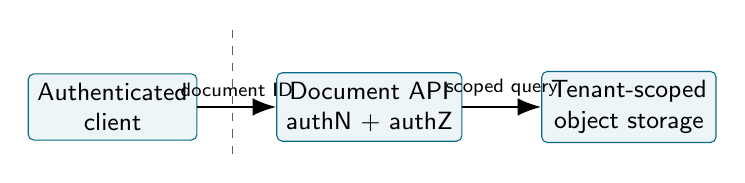
\begin{tikzpicture}[node distance=1.0cm and 1.0cm, every node/.style={font=\small}, box/.style={draw=accent,rounded corners=2pt,fill=pale,minimum height=0.75cm,align=center}]
\node[box] (u) {Authenticated\\client};
\node[box,right=of u] (a) {Document API\\authN + authZ};
\node[box,right=of a] (d) {Tenant-scoped\\object storage};
\draw[-{Latex[length=3mm]},thick] (u) -- node[above,font=\scriptsize] {document ID} (a);
\draw[-{Latex[length=3mm]},thick] (a) -- node[above,font=\scriptsize] {scoped query} (d);
\draw[dashed,muted] ($(a.west)+(-0.55,-0.6)$)--($(a.west)+(-0.55,1)$);
\end{tikzpicture}
\end{center}
\par\medskip\noindent\begin{tabularx}{\textwidth}{@{}p{0.2\textwidth}X@{}}\toprule
Element & Engineering result \\ \midrule
Abuse case & User of tenant A guesses document ID belonging to tenant B.\\
Precondition & Object lookup authorizes only login status, not resource ownership.\\
Requirement & Every read and write verifies principal--tenant--object relationship server-side.\\
Preventive check & Query constrains by authenticated tenant and object ID; deny by default.\\
Tests & Cross-tenant request returns 403/404 without object content; audit event recorded.\\
Residual risk & Misconfigured delegated sharing and inconsistent storage metadata.\\
\bottomrule\end{tabularx}\par\medskip
This example extends the web-authorization issues surveyed by the handbook and connects to OWASP API1:2023 (broken object-level authorization). \handbookref{10,79} \modernext{}

\section{Defense-in-depth and control placement}
A control should target an explicit failure mode. Avoid building a stack of tools that all depend on the same unverified identity provider or logging pipeline.
\par\medskip\noindent\begin{tabularx}{\textwidth}{@{}p{0.24\textwidth}X X@{}}\toprule
Layer & Preventive mechanism & Verification or detection \\ \midrule
Physical & Restricted access; tamper seals & Access log reviews; tamper inspections\\
Identity & MFA, least privilege, session policy & Impossible travel (with context); access review\\
Application & Explicit authorization, safe parsing & Security tests; SAST/DAST findings\\
Host & Patch management, constrained privilege & Endpoint telemetry, drift scans\\
Network & Default-deny segmentation, safe routing & Flow logs, network security monitoring\\
Data & AEAD, controlled keys, lifecycle rules & Key audit, unauthorized read tests\\
Recovery & Offline/immutable backups and playbooks & Restoration exercise, RTO measurements\\
\bottomrule\end{tabularx}\par\medskip
The handbook discusses layered defenses in network protection and enterprise security. A zero-trust implementation is a \emph{contemporary architecture strategy}, not a synonym for a purchased product. \handbookref{8,16,27} \modernext{}

\section{Risk statements and verification economics}
\subsection{Record risk in scenario form}\designed{}
Use: ``Because [precondition/weakness], [threat] may [event], causing [impact] to [asset/mission].'' Example: ``Because database read permission is shared among unrelated workloads, compromise of a low-trust worker may expose tenant documents.'' Assign owner, treatment, planned due date and proof of control performance.

\subsection{Separate findings, probabilities and proof}
A code scanner finding is evidence of a potential defect, not proof of remote exploitability. A blocked network path reduces exposure but does not erase vulnerable code. Prioritize by business impact, exploitation evidence, reachability, privilege, compensating controls and fix confidence. \handbookref{31,33,35} \modernext{}

\subsection{Assurance argument}\designed{}
\begin{enumerate}
\item \textbf{Claim:} cross-tenant object reads are blocked.
\item \textbf{Evidence:} unit and integration tests, policy decision traces, denied access logs.
\item \textbf{Warrant:} tests exercise each API path; storage query applies tenant constraints.
\item \textbf{Defeaters:} undiscovered admin endpoint or caching layer bypass.
\item \textbf{Disposition:} pass, conditional pass, remediate, or formally accept risk.
\end{enumerate}

\section{Knowledge checks and applied assessment}
\begin{enumerate}
\item Explain why strong encryption cannot compensate for authorization bypass.
\item Model a phishing attack in terms of asset, initial foothold, trust boundary, persistence and impact.
\item Classify full-packet capture as evidence, a detection enabler, or a preventive control; explain what it cannot demonstrate.
\item For a connected smart lock, identify one availability and one safety requirement distinct from confidentiality.
\item Write five threat statements for the document service; identify one verifiable control per threat.
\end{enumerate}
\begin{sourcebox}\textbf{Assessment rubric (100 points):} model completeness (20), plausible misuse conditions (25), controls traceable to threats (25), verification evidence (20), residual risk and explicit assumptions (10). A pass requires at least 80 points with no critical unmitigated design flaw. \designed{}\end{sourcebox}

\section*{Handbook chapter alignment}\addcontentsline{toc}{section}{Handbook chapter alignment}
These chapters ground the domain scope. The document offers original synthesis and technical procedures, not a chapter-by-chapter reproduction.
\par\medskip\noindent\begin{longtable}{@{}p{0.085\textwidth}p{0.68\textwidth}p{0.16\textwidth}@{}}\toprule Chapter & Handbook topic & Combined PDF p. \\ \midrule\endhead1 & Information Security in the Modern Enterprise & 39 \\
2 & Building a Secure Organization & 49 \\
4 & Verifying User and Host Identity & 83 \\
5 & Detecting System Intrusions & 91 \\
7 & Preventing System Intrusions & 157 \\
8 & Guarding Against Network Intrusions & 175 \\
14 & The Botnet Problem & 297 \\
19 & Security for the Internet of Things & 389 \\
24 & Information Security Essentials for IT Managers: Protecting Mission-Critical Systems & 459 \\
28 & The Enemy (The Intruder's Genesis) & 545 \\
29 & Social Engineering Deceptions and Defenses & 557 \\
36 & Insider Threats & 637 \\
71 & Physical Security & 1231 \\
79 & Access Controls & 1353 \\
88 & Cyber Attack Process & 1467 \\
89 & Smart Cities: Cybersecurity Concerns & 1483 \\
93 & An Overview of Cyber Attacks and Defenses on Intelligent Connected Vehicles & 1567 \\
102 & AI Abuse: Investigating the Threat Landscape & 1711 \\
\bottomrule\end{longtable}\par\medskip

\section*{Source and reference register}
\addcontentsline{toc}{section}{Source and reference register}
\begin{description}[leftmargin=1.6em,style=nextline]
\item[H] John R. Vacca (ed.), \emph{Computer and Information Security Handbook}, 4th ed., Volumes I--II, Elsevier/Morgan Kaufmann, 2025. Chapter identifiers in this document point to this book.
\item[N1] NIST, \emph{Cybersecurity Framework 2.0} (2024), \url{https://www.nist.gov/cyberframework}.
\item[N2] NIST SP 800-218, \emph{Secure Software Development Framework v1.1} (2022), \url{https://csrc.nist.gov/pubs/sp/800/218/final}. Later drafts are not treated as final requirements.
\item[N3] NIST SP 800-61 Rev. 3, \emph{Incident Response Recommendations and Considerations for Cybersecurity Risk Management} (2025), \url{https://csrc.nist.gov/pubs/sp/800/61/r3/final}.
\item[N4] NIST SP 800-63-4, \emph{Digital Identity Guidelines} (2025), \url{https://csrc.nist.gov/pubs/sp/800/63/4/final}.
\item[N5] NIST, FIPS 203/204/205 (2024), \url{https://csrc.nist.gov/Projects/Post-Quantum-Cryptography/publications}.
\item[O1] OWASP, \emph{API Security Top 10} (2023), \url{https://api-security.owasp.org/editions/2023/en/0x11-t10/}.
\item[C1] CISA, \emph{Known Exploited Vulnerabilities Catalog}, \url{https://www.cisa.gov/known-exploited-vulnerabilities-catalog}.
\item[M1] MITRE ATT\&CK Enterprise, \url{https://attack.mitre.org/matrices/enterprise/}.
\item[G1] GitHub, \emph{REST API endpoints for code scanning}, \url{https://docs.github.com/en/rest/code-scanning}.
\end{description}
\begin{warningbox}\textbf{Interpretation rule.} \handbookref{number} identifies a conceptual anchor in the supplied handbook, not a verbatim quotation or an official requirement. \modernext{} identifies a contemporary extension informed by external references or current engineering practice. \designed{} identifies an independently developed example, template, exercise, metric, or operational procedure. Requirements are binding only if separately adopted through applicable law, contract, policy, or the cited standards; this suite does not assert otherwise.\end{warningbox}

\end{document}
